\documentclass[11pt]{article}

\usepackage[spanish]{babel}
\usepackage[utf8]{inputenc}
\usepackage[T1]{fontenc}
\usepackage[margin=2.5cm]{geometry}
\usepackage{graphicx}
\usepackage{booktabs}
\usepackage{caption}
\usepackage{subcaption}
\usepackage{float}
\usepackage{amsmath}
\usepackage[hidelinks]{hyperref}

\setlength{\parindent}{1.5em}
\setlength{\parskip}{0pt}

\begin{document}

\begin{center}
{\LARGE Laboratorio 5: Clasificaci\'on de tweets usando miner\'ia de texto}\\[4pt]
{\large CC3084 -- Data Science, Semestre II 2026}
\end{center}

\vspace{0.8cm}

\begin{center}
Anthony Lou Schwank -- 23410 \\
Isabella Obando -- 23074 \\
Francisco Martinez -- 23617
\end{center}

\vspace{0.5cm}

\begin{center}
Repositorio del proyecto:\\
\texttt{https://github.com/Cisco890/lab5\_datascience}
\end{center}

\vspace{0.5cm}

\section{Introducci\'on}

El objetivo del laboratorio fue construir un clasificador capaz de determinar si un
tweet se refiere a un desastre real o no, usando el dataset \emph{Natural Language
Processing with Disaster Tweets} de Kaggle \cite{kaggle_disaster_tweets}. El trabajo
combin\'o miner\'ia de texto cl\'asica (limpieza, n-gramas, TF-IDF) con clasificaci\'on
supervisada y an\'alisis de sentimiento, y se organiz\'o en dos notebooks: uno de
avance (\texttt{lab5\_avances.ipynb}) con el an\'alisis exploratorio, el
preprocesamiento y el modelo preliminar, y uno de cierre
(\texttt{lab5\_clasificacion\_sentimiento.ipynb}) con la funci\'on de clasificaci\'on,
el an\'alisis de sentimiento y la variable de negatividad. Ambos reutilizan el mismo
pipeline de limpieza y entrenamiento, centralizado en \texttt{src/lab5\_pipeline.py}
para que los resultados sean reproducibles entre notebooks.

\section{Descripci\'on del conjunto de datos}

El conjunto de entrenamiento tiene \textbf{7{,}613 tweets} y 5 columnas: \texttt{id},
\texttt{keyword} (61 valores faltantes, 0.80\%), \texttt{location} (2{,}533 faltantes,
33.27\%), \texttt{text} (completo) y \texttt{target} (1 = desastre real, 0 = no). La
Figura~\ref{fig:missing} resume los faltantes por columna.

\begin{figure}[H]
\centering
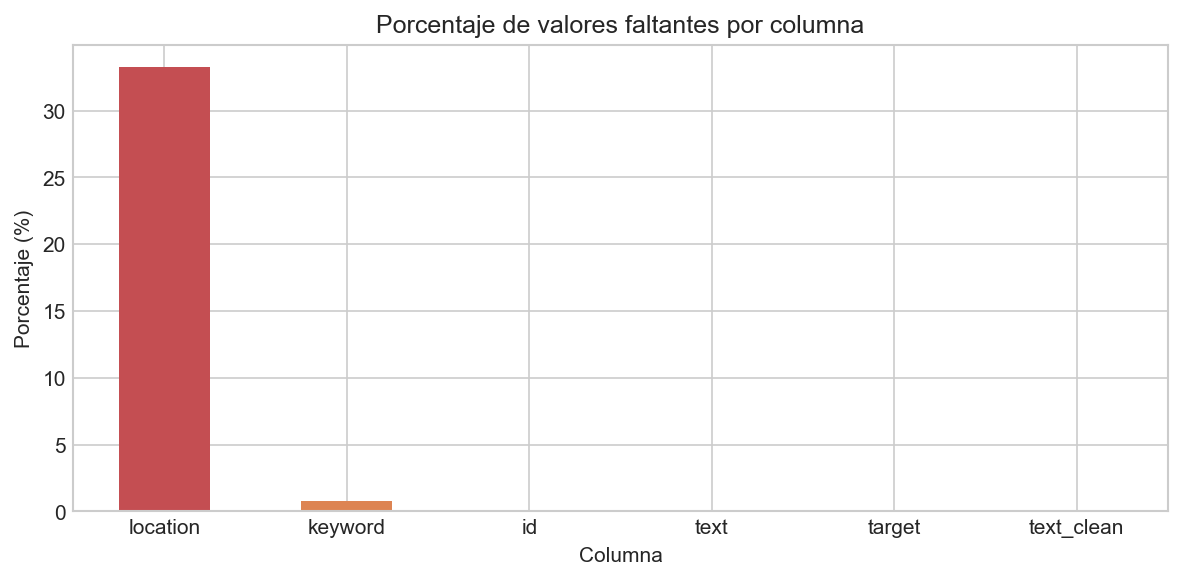
\includegraphics[width=0.7\textwidth]{figures/missing_values.png}
\caption{Porcentaje de valores faltantes por columna.}
\label{fig:missing}
\end{figure}

La variable objetivo muestra un desbalance moderado: \textbf{4{,}342 tweets (57.03\%)}
de clase 0 y \textbf{3{,}271 (42.97\%)} de clase 1 (Figura~\ref{fig:target}). No se
encontraron filas completamente duplicadas, aunque s\'i \textbf{110 textos repetidos},
que se conservaron para no alterar artificialmente la distribuci\'on del dataset.

\begin{figure}[H]
\centering
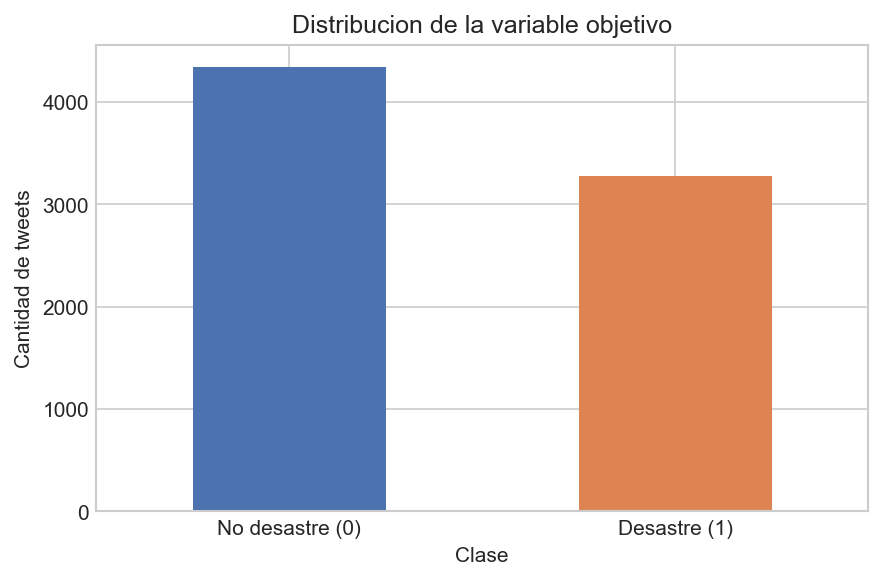
\includegraphics[width=0.55\textwidth]{figures/target_distribution.png}
\caption{Distribuci\'on de la variable objetivo.}
\label{fig:target}
\end{figure}

\section{Preprocesamiento y limpieza de texto}

La limpieza (funci\'on \texttt{limpiar\_texto}, implementada con \texttt{re} y
\texttt{scikit-learn}) aplic\'o, en orden: conversi\'on a min\'usculas; eliminaci\'on de
URLs y menciones \texttt{@usuario}; eliminaci\'on de emojis Unicode y emoticones de
texto (p.\ ej.\ \texttt{:)}); eliminaci\'on del s\'imbolo \texttt{\#} conservando la
palabra del hashtag; eliminaci\'on de signos de puntuaci\'on y apóstrofes; y
eliminaci\'on de \emph{stopwords} en ingl\'es (\texttt{ENGLISH\_STOP\_WORDS} de
\texttt{scikit-learn}). Los n\'umeros se conservaron deliberadamente: aunque la mayor\'ia
son gen\'ericos, casos como \texttt{911} aparecen asociados a emergencias reales.

Antes de decidir qu\'e hacer con los emoticones se cuantific\'o su presencia: no se
encontr\'o \textbf{ning\'un} tweet con emoji Unicode real, y solo \textbf{82 tweets}
(1.1\% del dataset) con emoticones de texto, sin diferencia relevante entre clases. Por
eso se eliminaron de \texttt{text\_clean} (el texto usado por el modelo de bolsa de
palabras), pero se conserv\'o el texto original sin modificar para el an\'alisis de
sentimiento de la Secci\'on~\ref{sec:sentimiento}, donde s\'i pueden aportar se\~nal.
Tras la limpieza completa solo \textbf{4 textos} quedaron vac\'ios, lo que indica que el
preprocesamiento no fue demasiado agresivo.

\section{An\'alisis exploratorio}

Los tweets de desastre real tienden a ser ligeramente m\'as largos (108.1 caracteres en
promedio vs.\ 95.7 en la otra clase) y a incluir m\'as URLs (0.77 vs.\ 0.51 en promedio),
mientras que las menciones son m\'as frecuentes en tweets no-desastre
(Figura~\ref{fig:boxplots}). Estas diferencias existen pero no son lo bastante fuertes
como para separar las clases por s\'i solas, por lo que la se\~nal principal debe venir
del contenido l\'exico del texto.

\begin{figure}[H]
\centering
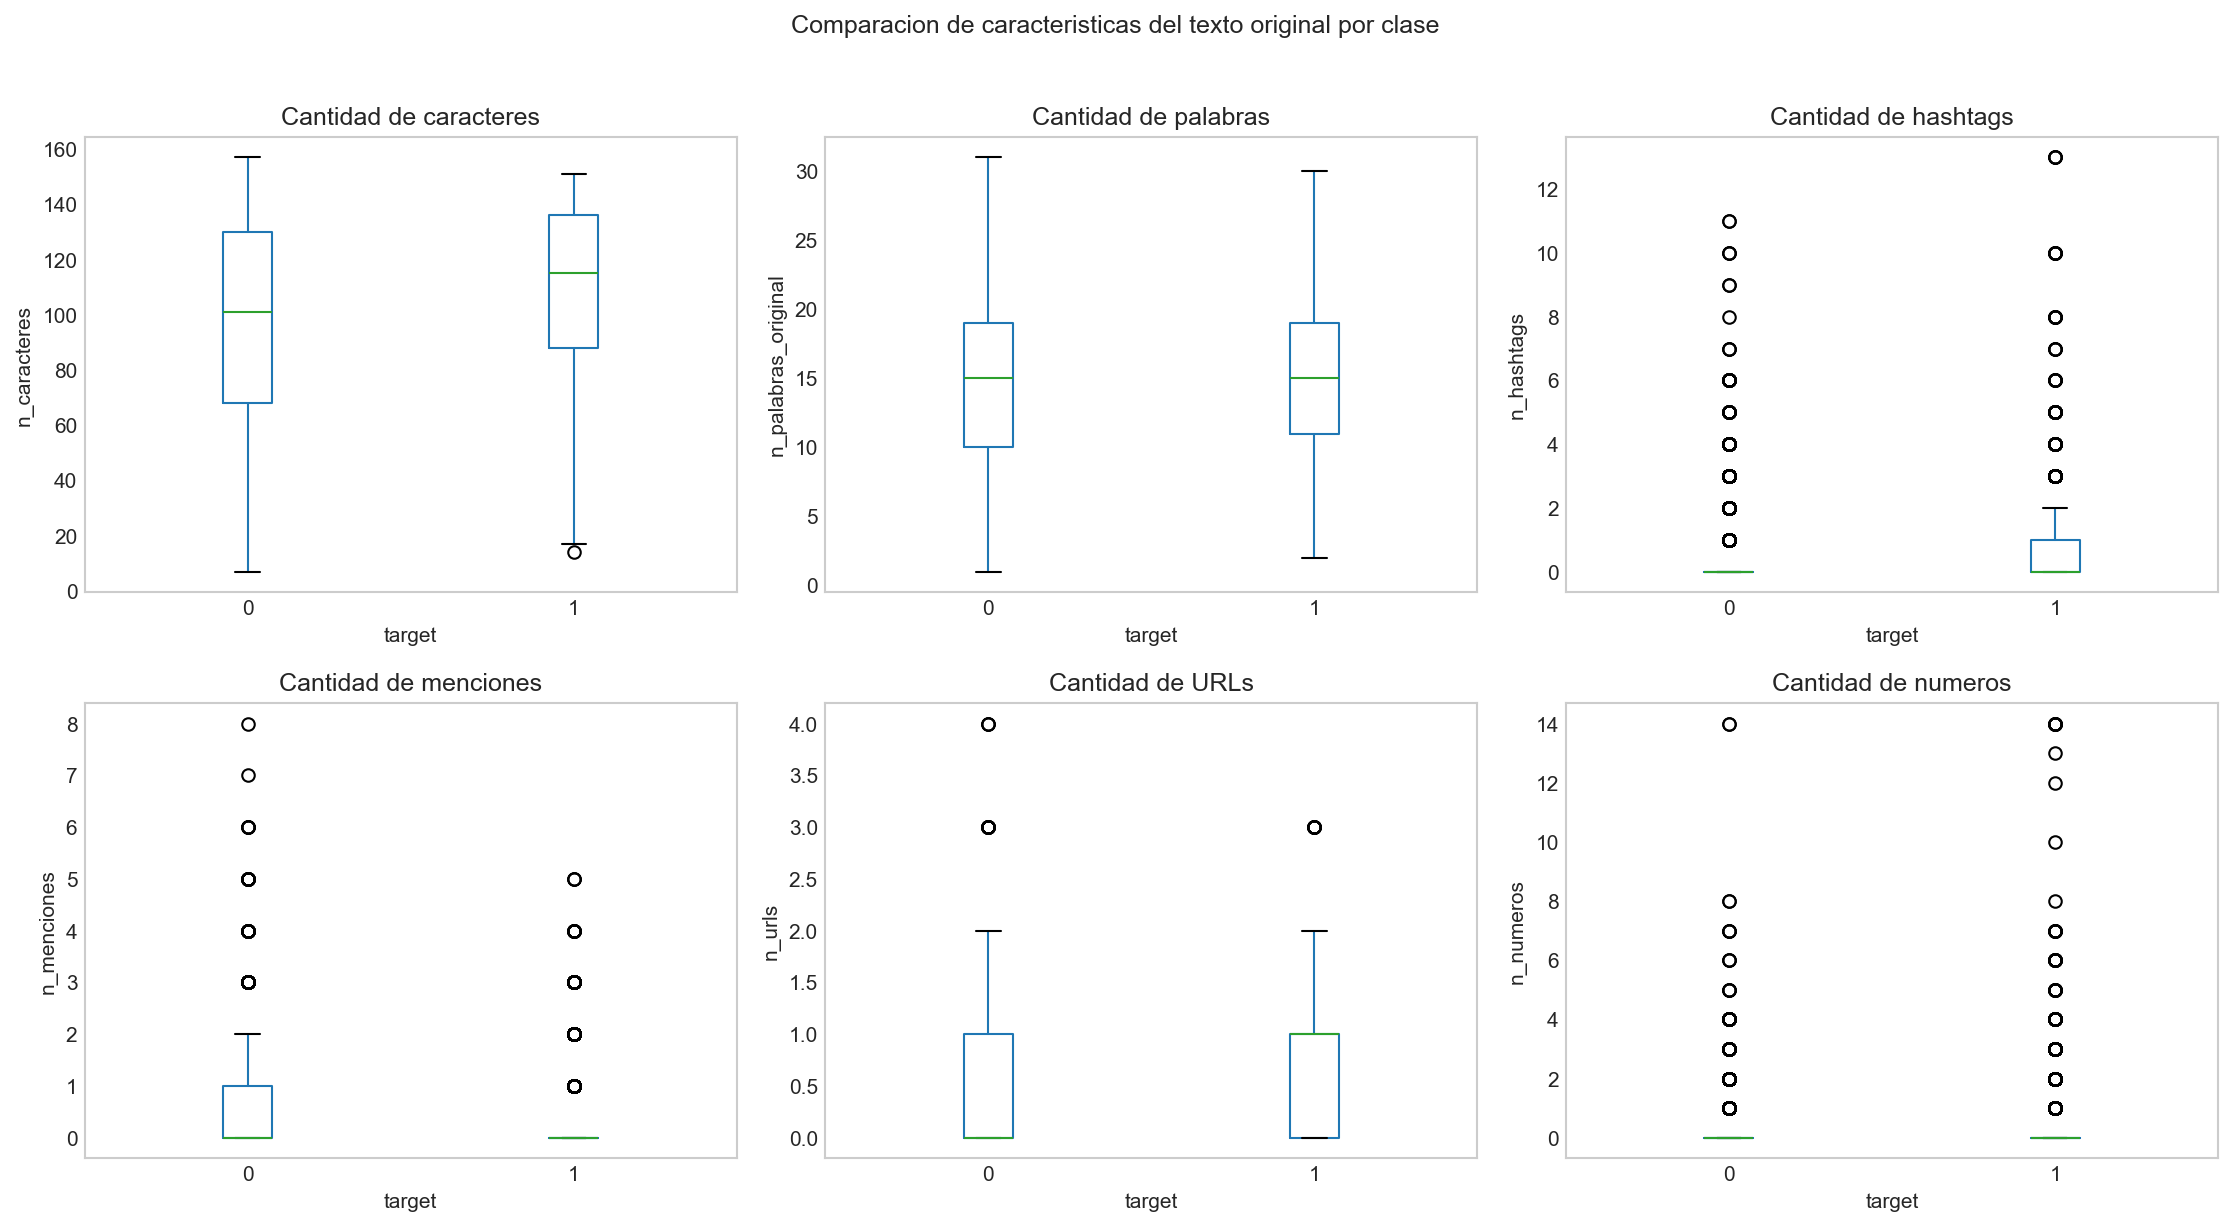
\includegraphics[width=\textwidth]{figures/text_features_boxplots.png}
\caption{Caracter\'isticas del texto original por clase.}
\label{fig:boxplots}
\end{figure}

\subsection{Frecuencia de unigramas y bigramas}

La Figura~\ref{fig:unigramas} muestra los 20 unigramas m\'as frecuentes por clase.
Palabras como \texttt{like}, \texttt{just} o \texttt{new} dominan en tweets no-desastre,
mientras que \texttt{news}, \texttt{disaster}, \texttt{california} y \texttt{suicide}
dominan en tweets de desastre real. Sin embargo, varias palabras frecuentes
(\texttt{amp}, \texttt{people}, \texttt{time}) aparecen en ambas categor\'ias, lo que
muestra que la frecuencia aislada no basta para separar clases.

\begin{figure}[H]
\centering
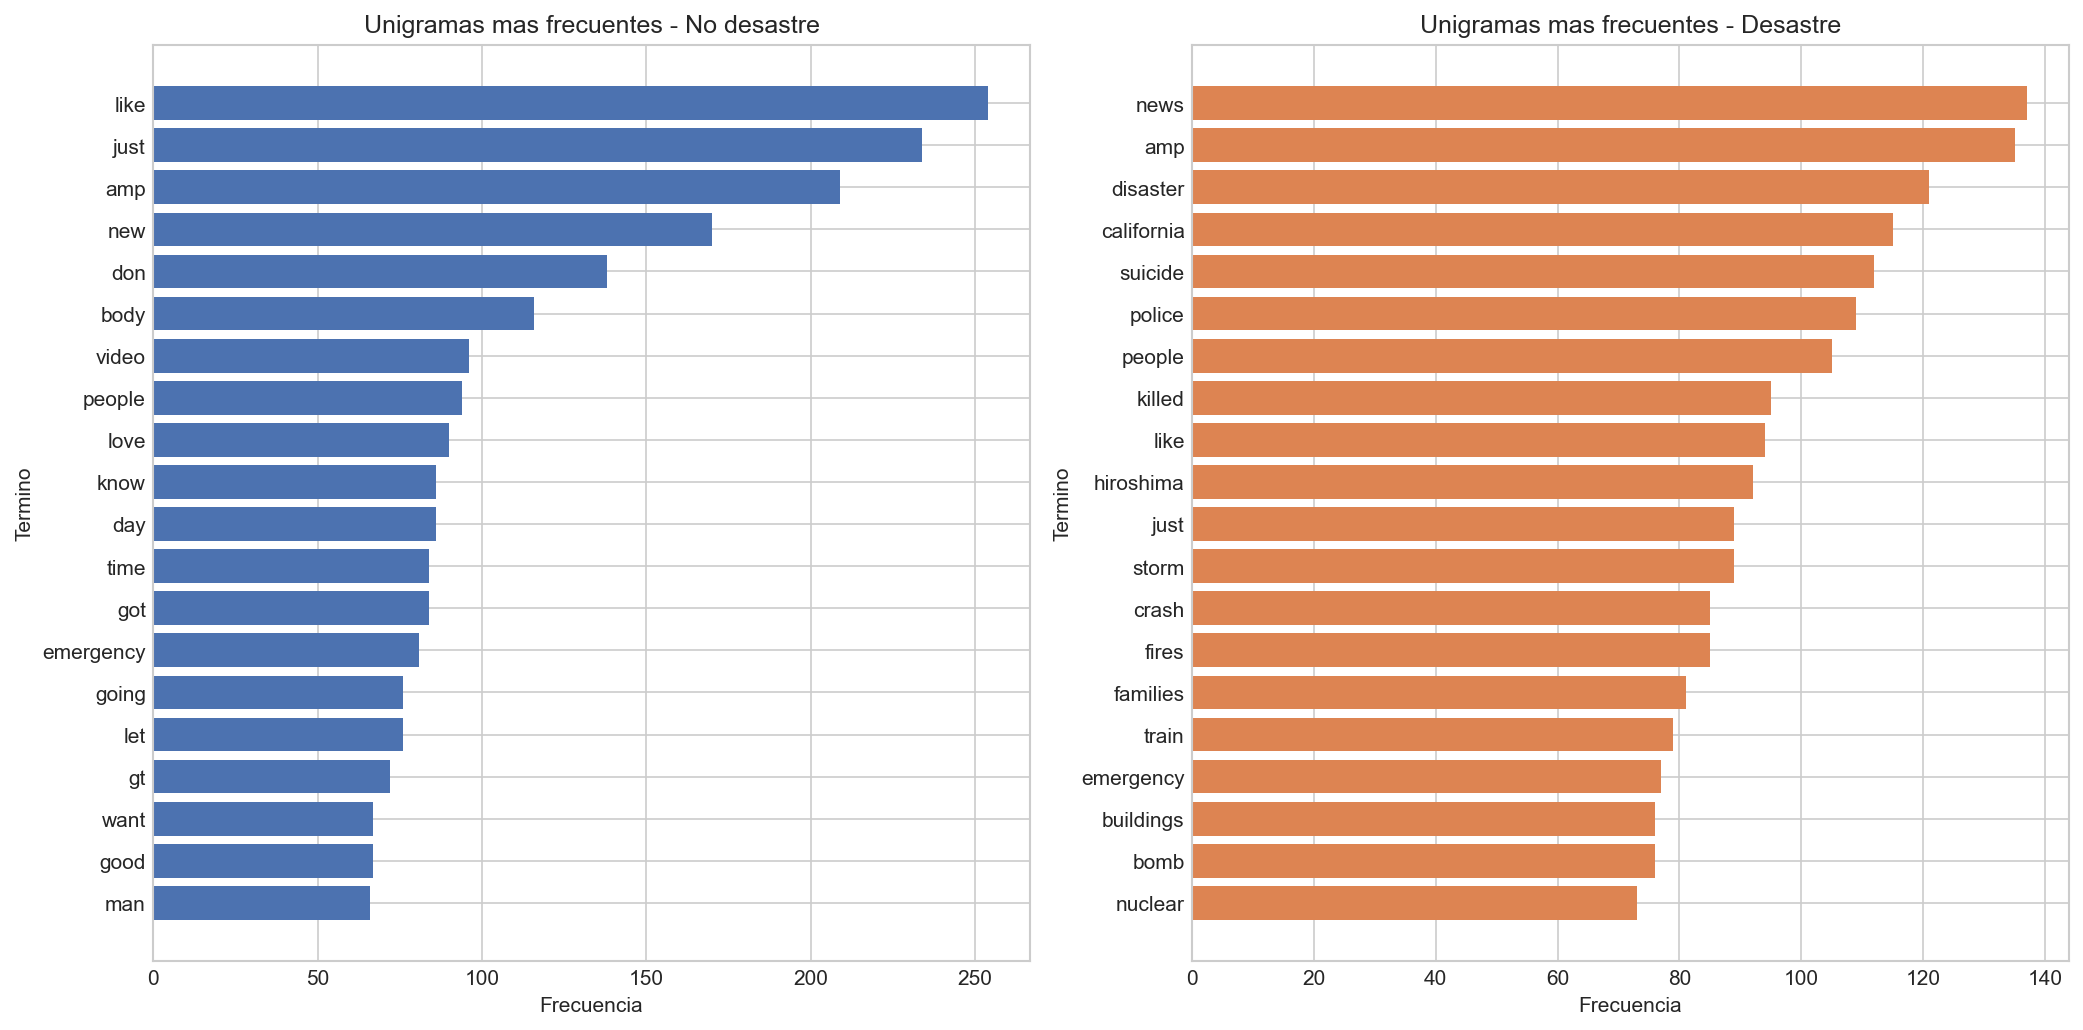
\includegraphics[width=\textwidth]{figures/unigramas_por_clase.png}
\caption{Unigramas m\'as frecuentes por clase.}
\label{fig:unigramas}
\end{figure}

Los bigramas (Figura~\ref{fig:bigramas}) s\'i aportan contexto adicional: expresiones
como \texttt{suicide bomber}, \texttt{california wildfire} u \texttt{oil spill} son
casi exclusivas de tweets de desastre real, mientras que combinaciones como
\texttt{cross body} o \texttt{liked video} son t\'ipicas de la otra clase (p.\ ej.\
tweets sobre bolsos/moda o notificaciones autom\'aticas de redes sociales, no sobre
desastres). Se explor\'o tambi\'en un nivel de trigramas, pero con textos tan cortos
como los tweets su frecuencia cae r\'apido y aportan pocas frases nuevas, por lo que se
dejaron como an\'alisis exploratorio y no como parte del modelo.

\begin{figure}[H]
\centering
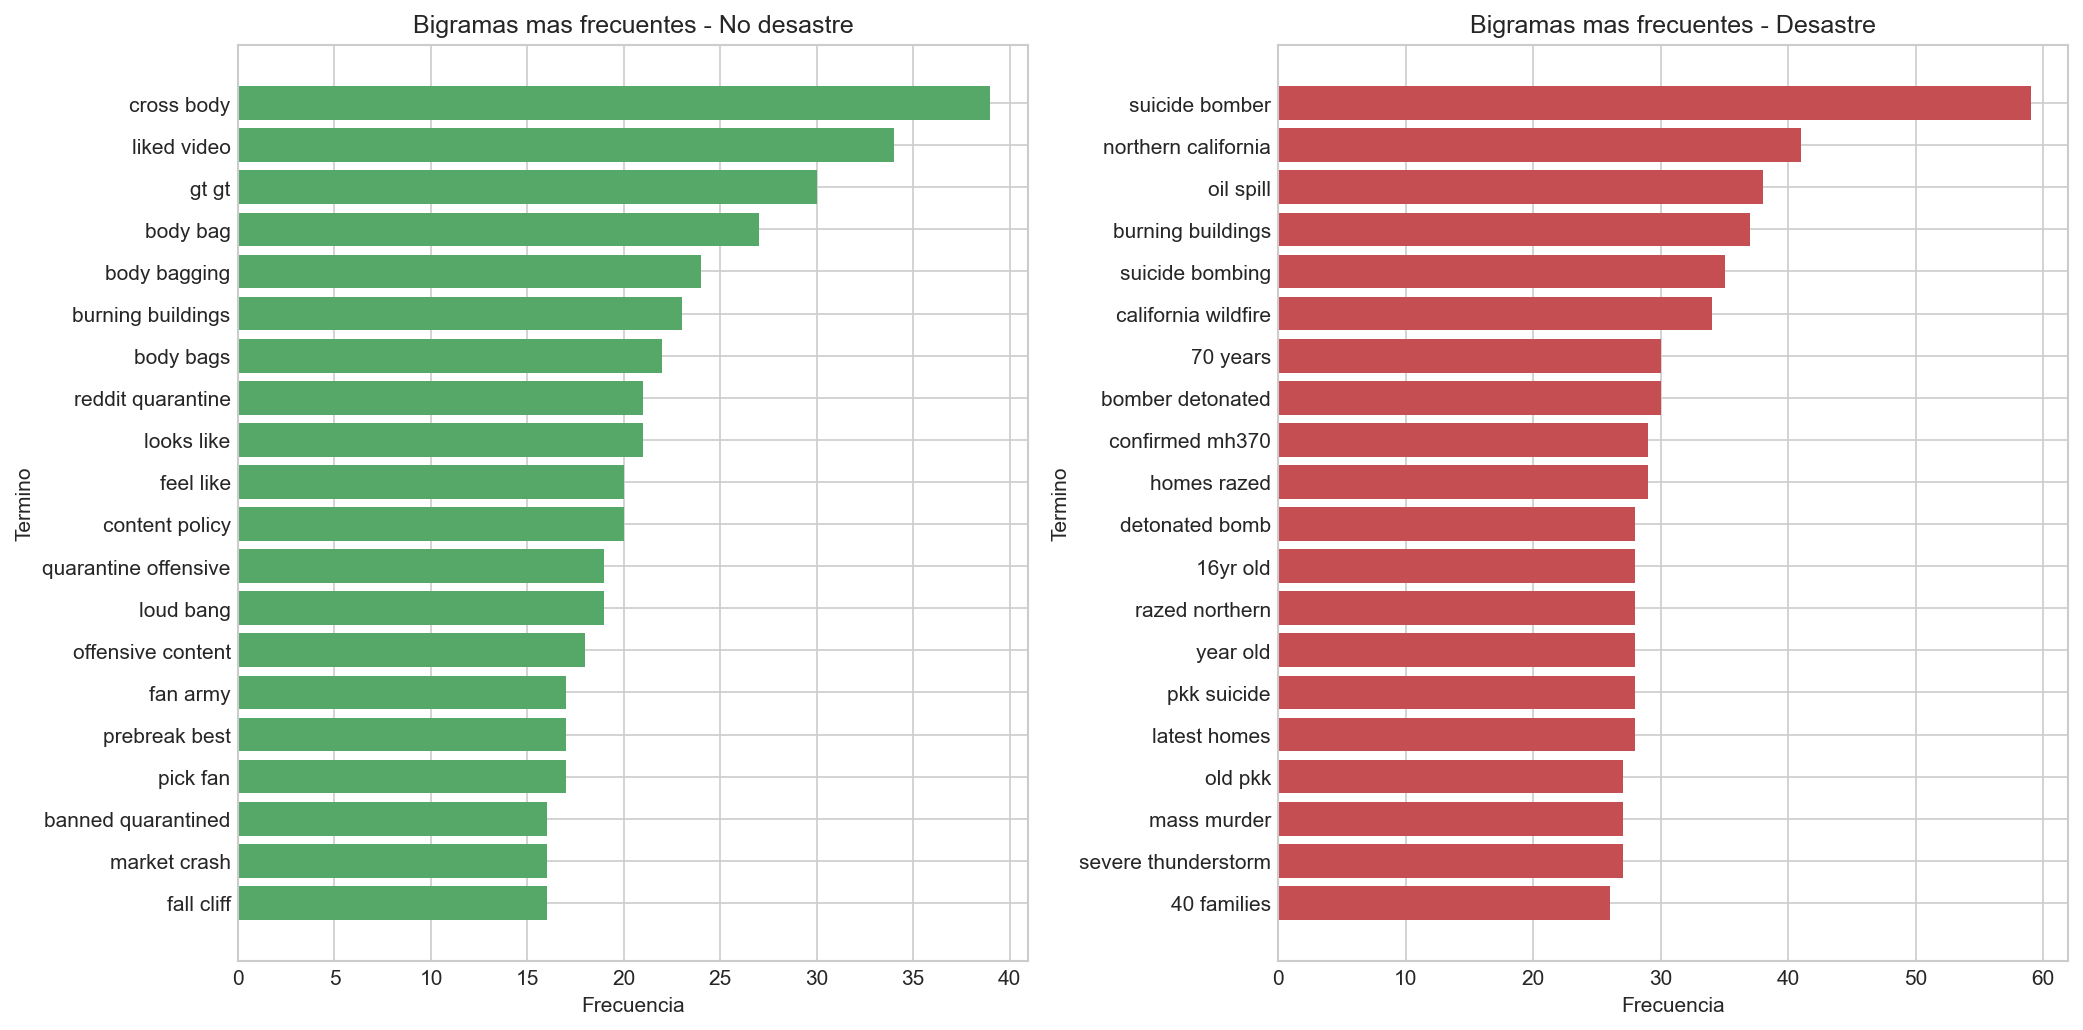
\includegraphics[width=\textwidth]{figures/bigramas_por_clase.png}
\caption{Bigramas m\'as frecuentes por clase.}
\label{fig:bigramas}
\end{figure}

\subsection{Nube de palabras}

La Figura~\ref{fig:wordcloud} visualiza el mismo vocabulario de forma cualitativa. En la
nube de ``desastre'' resaltan t\'erminos como \texttt{disaster}, \texttt{suicide},
\texttt{california}, \texttt{police} y \texttt{killed}; en la de ``no desastre''
resaltan \texttt{love}, \texttt{video}, \texttt{time} y \texttt{new}. Palabras como
\texttt{amp} y \texttt{new} aparecen grandes en ambas, lo que confirma la ambig\"uedad ya
detectada en las tablas de frecuencia.

\begin{figure}[H]
\centering
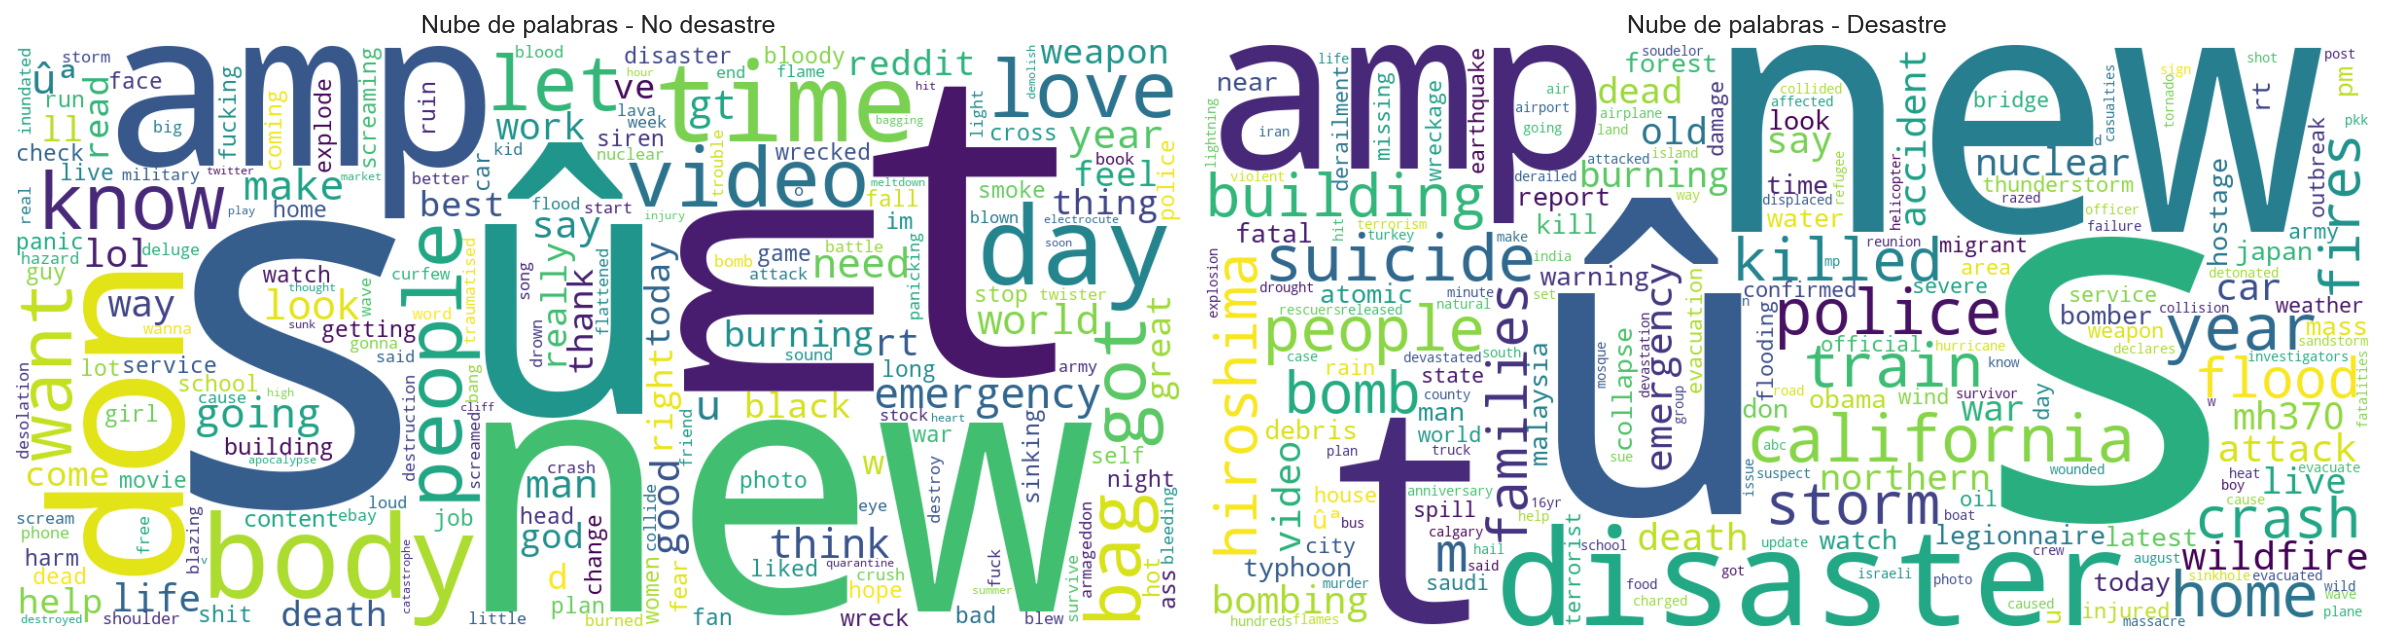
\includegraphics[width=\textwidth]{figures/wordcloud.png}
\caption{Nube de palabras por clase (generada con la librer\'ia \texttt{wordcloud}).}
\label{fig:wordcloud}
\end{figure}

\subsection{Probabilidades de n-gramas por clase}

Para complementar las frecuencias con una medida de probabilidad, se calcul\'o, para
cada uno de los 20 unigramas y 20 bigramas globales m\'as frecuentes, la proporci\'on de
tweets de cada clase que lo contienen ($P(\text{t\'ermino}\mid\text{desastre})$ y
$P(\text{t\'ermino}\mid\text{no desastre})$) y su raz\'on de verosimilitud en escala
logar\'itmica (\emph{log-odds}) --la misma l\'ogica que usa internamente un
clasificador Naive Bayes. La Figura~\ref{fig:logodds} muestra el resultado ordenado de
menor a mayor \emph{log-odds}.

\begin{figure}[H]
\centering
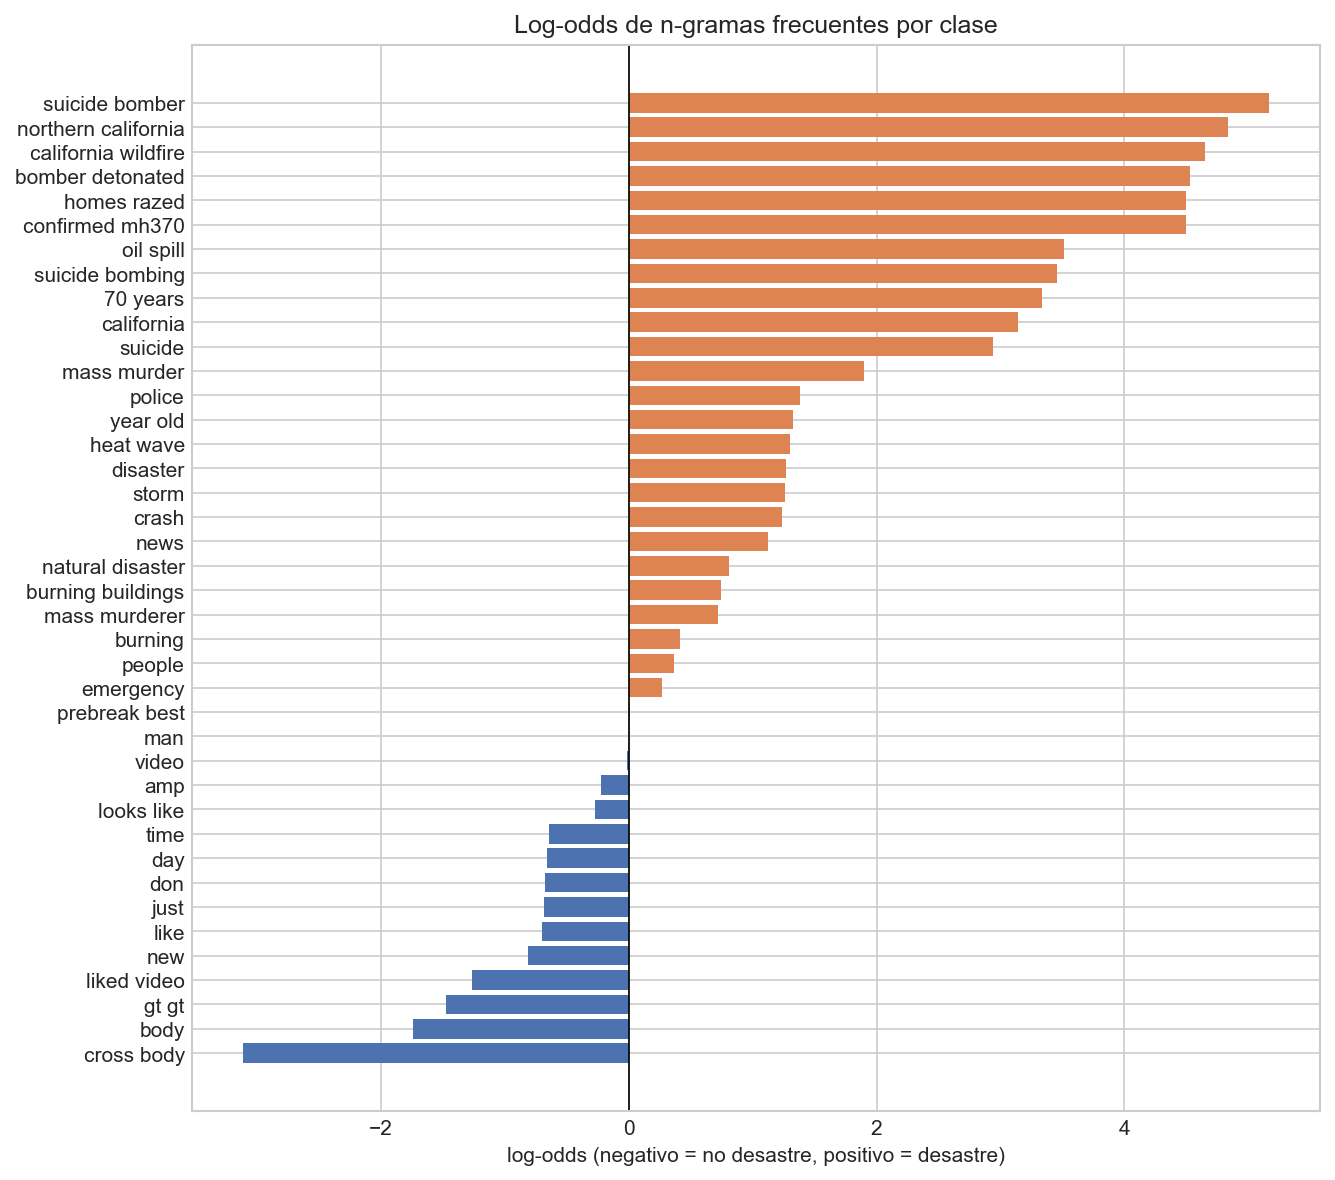
\includegraphics[width=0.75\textwidth]{figures/log_odds_ngramas.png}
\caption{Log-odds de n-gramas frecuentes por clase.}
\label{fig:logodds}
\end{figure}

El t\'ermino m\'as exclusivo de ``desastre'' fue \texttt{suicide bomber}
($P=1.74\%$ vs.\ $0.00\%$), y el m\'as exclusivo de ``no desastre'' fue
\texttt{cross body} ($P=0.90\%$ vs.\ $0.03\%$, proveniente de tweets sobre bolsos y
moda que usan la palabra \texttt{body} sin relaci\'on con desastres). Los t\'erminos con
\emph{log-odds} cercano a 0 (\texttt{amp}, \texttt{video}) son frecuentes en ambas clases
y por s\'i solos aportan poca capacidad discriminativa.

\subsection{Variable \texttt{keyword}}

La columna \texttt{keyword} resume un tema expl\'icito del tweet y muestra proporciones
de clase muy variables: \texttt{derailment} y \texttt{wreckage} son 100\% desastre real,
mientras que \texttt{aftershock} es 0\%. Es una variable interpretable, pero con ruido
suficiente (algunas keywords aparecen en ambos contextos) como para no incorporarla
todav\'ia en el modelo de texto puro.

\section{Modelos de clasificaci\'on}

\subsection{Representaci\'on y algoritmo principal}

Como representaci\'on se us\'o \textbf{TF-IDF} (\texttt{TfidfVectorizer} de
\texttt{scikit-learn}, \texttt{min\_df=2}, \texttt{max\_df=0.95}) sobre
\texttt{text\_clean}, ajustada \'unicamente con el 80\% de entrenamiento
(\texttt{train\_test\_split}, \texttt{stratify=y}, \texttt{random\_state=42}) para
evitar fuga de informaci\'on. El algoritmo principal fue \textbf{Regresi\'on
Log\'istica} (\texttt{max\_iter=1000}), elegida por su simplicidad, velocidad e
interpretabilidad para datos de texto dispersos.

\begin{table}[H]
\centering
\caption{Comparaci\'on de representaciones (Regresi\'on Log\'istica).}
\begin{tabular}{lrrrr}
\toprule
Representaci\'on & Accuracy & Precision & Recall & F1 \\
\midrule
Unigramas & 0.8227 & 0.8516 & 0.7110 & 0.7750 \\
Unigramas + bigramas & \textbf{0.8234} & \textbf{0.8519} & \textbf{0.7125} & \textbf{0.7760} \\
\bottomrule
\end{tabular}
\end{table}

Agregar bigramas mejor\'o marginalmente todas las m\'etricas, por lo que se conserv\'o
la representaci\'on unigramas + bigramas para el resto del an\'alisis.

\subsection{Comparaci\'on de algoritmos}

Para cumplir con probar var\'ios algoritmos, se entren\'o adem\'as un \textbf{Naive
Bayes Multinomial} sobre la misma representaci\'on. La Tabla~\ref{tab:algoritmos} y la
Figura~\ref{fig:confusion} resumen la comparaci\'on.

\begin{table}[H]
\centering
\caption{Comparaci\'on de algoritmos de clasificaci\'on.}
\label{tab:algoritmos}
\begin{tabular}{lrrrr}
\toprule
Algoritmo & Accuracy & Precision & Recall & F1 \\
\midrule
Regresi\'on Log\'istica & \textbf{0.8234} & 0.8519 & \textbf{0.7125} & \textbf{0.7760} \\
Naive Bayes Multinomial & 0.8155 & \textbf{0.8621} & 0.6789 & 0.7596 \\
\bottomrule
\end{tabular}
\end{table}

\begin{figure}[H]
\centering
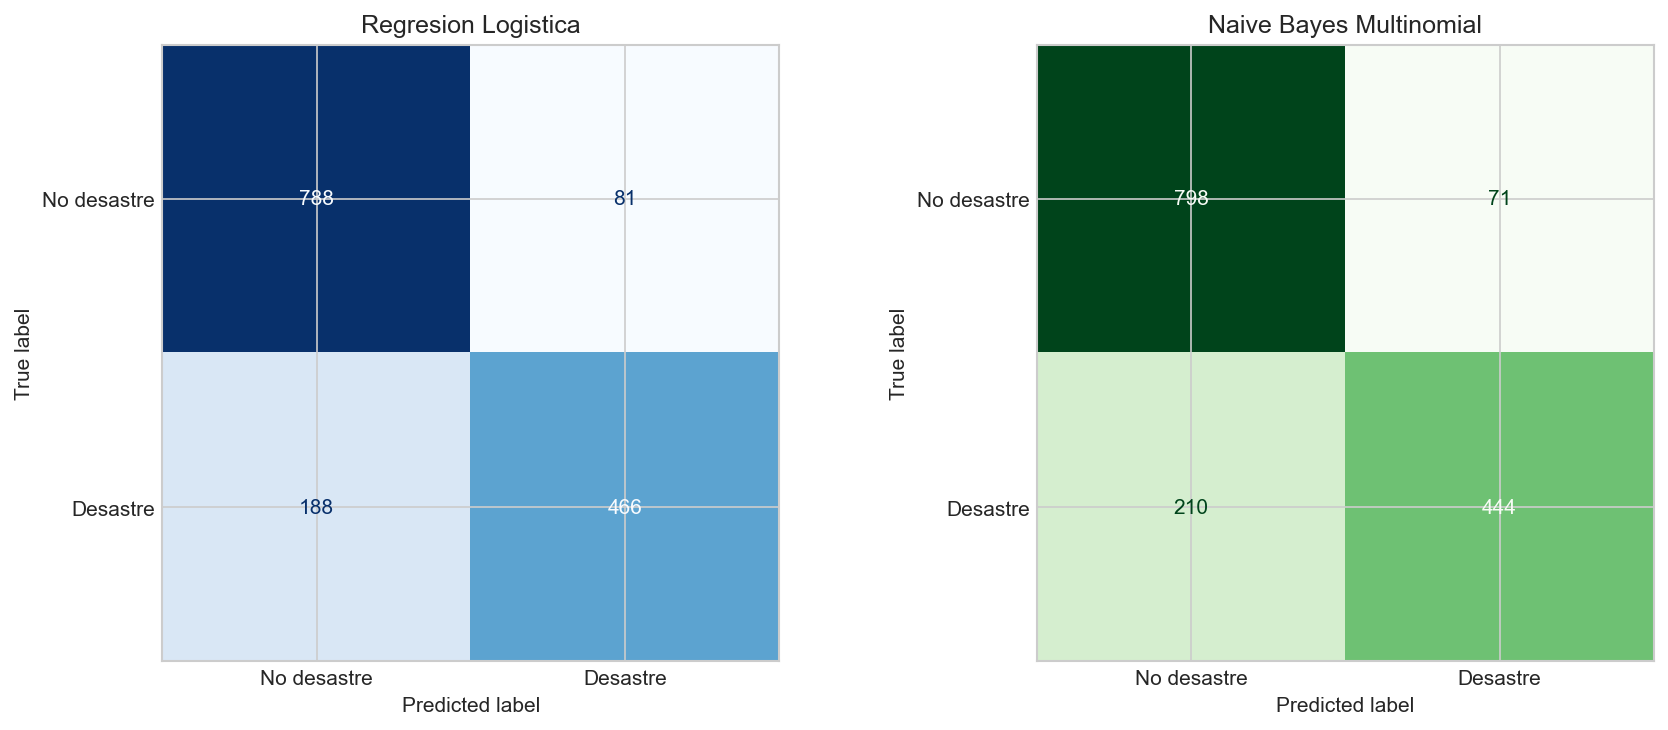
\includegraphics[width=\textwidth]{figures/matrices_confusion.png}
\caption{Matrices de confusi\'on: Regresi\'on Log\'istica y Naive Bayes Multinomial.}
\label{fig:confusion}
\end{figure}

Naive Bayes tiene mejor \emph{precision} pero peor \emph{recall}: su suposici\'on de
independencia entre palabras es una simplificaci\'on fuerte cuando el contexto importa
(distinguir bigramas con significado literal de uno figurado). La Regresi\'on
Log\'istica, al permitir regularizaci\'on y no asumir esa independencia, obtuvo mejor
F1 global y se seleccion\'o como \textbf{modelo final} para el resto del an\'alisis
(funci\'on de clasificaci\'on, interpretaci\'on de coeficientes y variable de
negatividad).

Los coeficientes de la Regresi\'on Log\'istica confirman los mismos patrones que el
an\'alisis de \emph{log-odds}: t\'erminos como \texttt{hiroshima}, \texttt{california},
\texttt{fires} y \texttt{killed} tienen los coeficientes m\'as altos hacia
``desastre'', mientras que \texttt{love}, \texttt{new} y \texttt{let} son los m\'as
fuertes hacia ``no desastre''. Al revisar una muestra de errores, la mayor\'ia
corresponde a tweets ambiguos, cortos o con uso figurado del vocabulario, dif\'iciles
de resolver con una representaci\'on de bolsa de palabras.

\section{Funci\'on de clasificaci\'on}

Se implement\'o \texttt{clasificar\_tweet(texto)}, que recibe el \textbf{texto crudo
de un tweet, sin preprocesar}, aplica internamente la misma limpieza y el mismo
vectorizador TF-IDF del modelo entrenado, y devuelve la etiqueta predicha junto con la
probabilidad asociada. La Tabla~\ref{tab:ejemplos_clasificacion} muestra ejemplos con
may\'usculas, menciones, URLs y hashtags sin procesar.

\begin{table}[H]
\centering
\caption{Ejemplos de clasificaci\'on con texto crudo.}
\label{tab:ejemplos_clasificacion}
\small
\begin{tabular}{p{9.5cm}ll}
\toprule
Tweet (texto crudo) & Etiqueta & Prob. \\
\midrule
BREAKING: Massive 7.2 earthquake hits California... & Desastre & 90.2\% \\
This traffic jam... is an absolute disaster... lol & Desastre & 52.9\% \\
Forest fire spreading fast near the city... & Desastre & 81.9\% \\
I'm on fire today, nailed every presentation... & No desastre & 67.9\% \\
Just watched a documentary about the 2004 tsunami... & No desastre & 70.7\% \\
@user CAN YOU BELIEVE this flood destroyed... & No desastre & 56.2\% \\
\bottomrule
\end{tabular}
\end{table}

El modelo distingue correctamente los usos figurados m\'as evidentes (``I'm on fire
today'' sobre una buena jornada de trabajo), aunque casos ambiguos como el uso
coloquial de ``disaster'' para describir tr\'afico quedan cerca del umbral de decisi\'on
(52.9\%), reflejando la dificultad ya observada en el an\'alisis de errores.

\section{An\'alisis de sentimiento}
\label{sec:sentimiento}

Para determinar si un tweet es positivo, negativo o neutro se us\'o \textbf{VADER}
(\emph{Valence Aware Dictionary and sEntiment Reasoner}) \cite{vader2014}, disponible en
\texttt{nltk.sentiment} --uno de los m\'odulos sugeridos en el enunciado. VADER es un
analizador basado en l\'exico dise\~nado espec\'ificamente para texto de redes sociales:
cada palabra tiene un puntaje de valencia, y el puntaje agregado (\texttt{compound},
entre $-1$ y $1$) pondera adem\'as may\'usculas, signos de exclamaci\'on, negaciones e
intensificadores. Se clasific\'o cada tweet como positivo si \texttt{compound}
$\geq 0.05$, negativo si $\leq -0.05$, y neutro en otro caso (umbral recomendado por la
documentaci\'on oficial de VADER).

A diferencia de \texttt{text\_clean}, para este an\'alisis se us\'o una limpieza
liviana que solo elimina URLs y menciones, \textbf{conservando} may\'usculas,
puntuaci\'on y emoticones, ya que son se\~nales que el l\'exico de VADER usa
expl\'icitamente.

\begin{figure}[H]
\centering
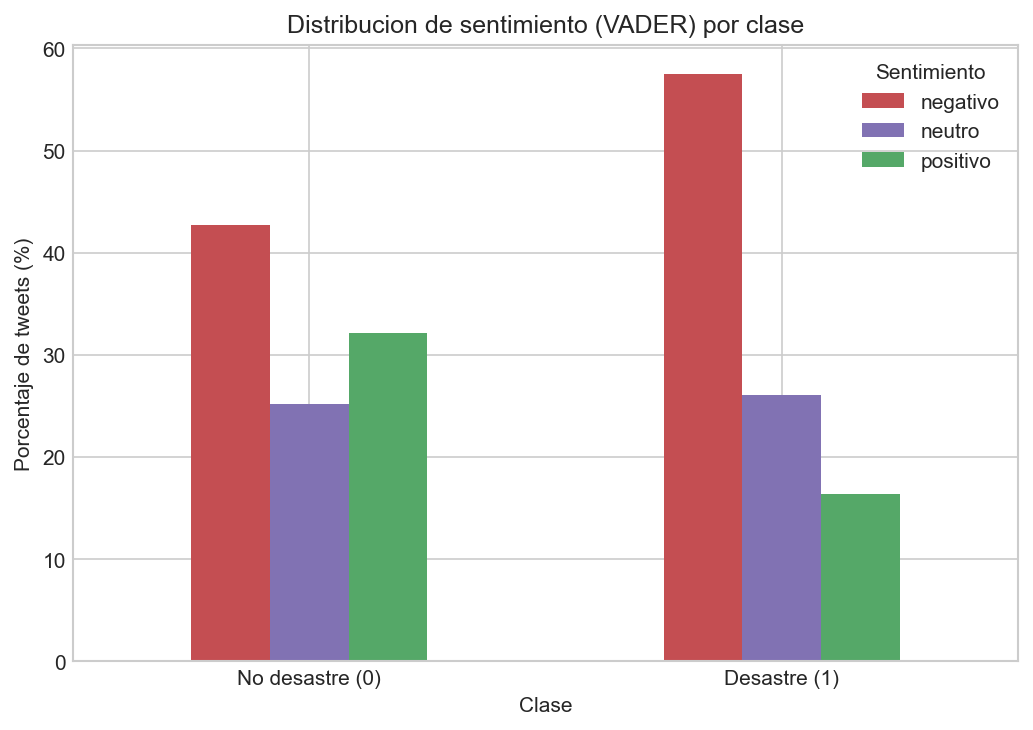
\includegraphics[width=0.7\textwidth]{figures/sentimiento_por_clase.png}
\caption{Distribuci\'on de sentimiento (VADER) por clase.}
\label{fig:sentimiento}
\end{figure}

Como muestra la Figura~\ref{fig:sentimiento}, los tweets de desastre real son
\textbf{57.5\% negativos}, frente a \textbf{42.7\%} en la otra clase; el patr\'on
inverso ocurre con los positivos (16.4\% vs.\ 32.1\%).

\section{Resultados}

\subsection{Tweets m\'as negativos y m\'as positivos}

De los \textbf{10 tweets m\'as negativos} seg\'un VADER, \textbf{8 pertenecen a la
categor\'ia ``Desastre''}: tem\'aticamente son atentados, bombas suicidas y ataques con
v\'ictimas mortales, vocabulario que VADER capta como muy negativo tanto por las
palabras (\texttt{killed}, \texttt{suicide bomber}, \texttt{dead}) como por se\~nales
de \'enfasis (may\'usculas, repetici\'on, signos de exclamaci\'on). De los \textbf{10
tweets m\'as positivos}, \textbf{8 pertenecen a ``No desastre''}: predominan tweets
sobre entretenimiento, agradecimientos o buenos deseos (\texttt{love},
\texttt{happy}, \texttt{great}).

\subsection{¿Son los tweets de desastre real m\'as negativos?}

S\'i: el promedio de \texttt{vader\_compound} es $-0.2668$ para tweets de desastre real
frente a $-0.0565$ para el resto, y una prueba $t$ de Welch confirma que la diferencia
es estad\'isticamente significativa ($p < 0.05$). Esto es consistente con lo observado
en la Secci\'on~\ref{sec:sentimiento} y con el hecho de que los tweets sobre desastres
reales describen muertes, destrucci\'on y emergencias, mientras que el uso figurado del
vocabulario de desastre aparece m\'as en contextos cotidianos o positivos.

\subsection{Variable de negatividad y reentrenamiento}

Se defini\'o \texttt{negatividad} $= -\texttt{vader\_compound}$ (rango $[-1,1]$, valores
altos = tweet m\'as negativo) y se agreg\'o como columna num\'erica adicional a la
matriz TF-IDF (\texttt{scipy.sparse.hstack}), estandarizada con \texttt{StandardScaler}
ajustado solo con el conjunto de entrenamiento. La Figura~\ref{fig:negatividad} muestra
que, en efecto, la distribuci\'on de negatividad es m\'as alta en tweets de desastre
real.

\begin{figure}[H]
\centering
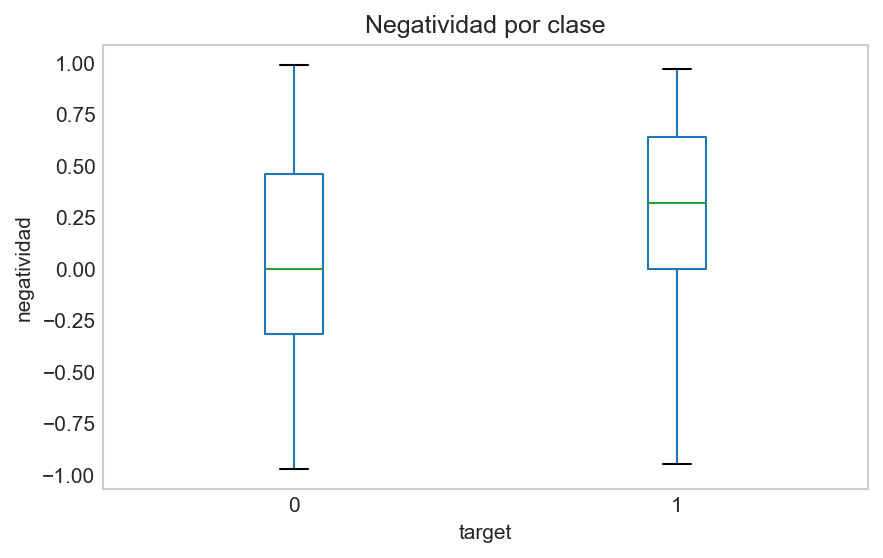
\includegraphics[width=0.55\textwidth]{figures/negatividad_por_clase.png}
\caption{Negatividad por clase.}
\label{fig:negatividad}
\end{figure}

\begin{table}[H]
\centering
\caption{Efecto de agregar la variable de negatividad al modelo.}
\begin{tabular}{lrrrr}
\toprule
Modelo & Accuracy & Precision & Recall & F1 \\
\midrule
Base (solo TF-IDF) & \textbf{0.8234} & \textbf{0.8519} & 0.7125 & \textbf{0.7760} \\
+ negatividad & 0.8188 & 0.8399 & \textbf{0.7141} & 0.7719 \\
\bottomrule
\end{tabular}
\end{table}

El resultado honesto es que \textbf{incluir la negatividad no mejor\'o el modelo}: el
F1 baj\'o de 0.7760 a 0.7719 (accuracy y precision tambi\'en bajan levemente; solo el
recall sube 0.0016). Esto es razonable: la negatividad resume todo el tweet en un solo
n\'umero, mientras que la representaci\'on TF-IDF con miles de t\'erminos ya captura
se\~nales mucho m\'as espec\'ificas (palabras casi in\'equ\'ivocas de una clase, como
\texttt{hiroshima} o \texttt{wildfire}, que ninguna medida de sentimiento general puede
replicar). El sentimiento negativo de un tweet ya est\'a correlacionado con varias de
esas palabras que el TF-IDF tambi\'en ve, as\'i que la variable aporta poca informaci\'on
nueva y, en este caso, ni compensa el ruido adicional que introduce.

\section{Limitaciones}

El dataset tiene 110 textos repetidos y algunos caracteres corruptos (secuencias como
\texttt{Û\_}) provenientes de una codificaci\'on inconsistente en el origen de los
datos, que no se corrigieron por no afectar de forma relevante el vocabulario m\'as
frecuente. El umbral de sentimiento de VADER ($\pm 0.05$) es el recomendado por la
librer\'ia, pero no fue calibrado espec\'ificamente para este dominio (tweets de
desastres). La variable \texttt{keyword}, con potencial predictivo, no se incorpor\'o
todav\'ia al modelo final. Finalmente, la comparaci\'on de algoritmos se limit\'o a dos
familias (Regresi\'on Log\'istica y Naive Bayes); otros algoritmos (p.\ ej.\ SVM lineal
o \emph{gradient boosting}) podr\'ian mejorar a\'un m\'as el resultado.

\section{Conclusiones}

El texto limpio (\texttt{text\_clean}) con representaci\'on TF-IDF (unigramas +
bigramas) y Regresi\'on Log\'istica alcanz\'o \textbf{Accuracy = 0.8234},
\textbf{Precision = 0.8519}, \textbf{Recall = 0.7125} y \textbf{F1 = 0.7760} en el
conjunto de prueba, superando a Naive Bayes Multinomial (F1 = 0.7596). El an\'alisis de
n-gramas y de \emph{log-odds} identific\'o t\'erminos casi exclusivos de cada clase
(\texttt{suicide bomber} para desastre, \texttt{cross body} para no desastre), pero
tambi\'en mostr\'o que buena parte del vocabulario frecuente es ambiguo y depende del
contexto, lo que justifica el uso de bigramas. El an\'alisis de sentimiento con VADER
confirm\'o, de forma estad\'isticamente significativa, que los tweets de desastre real
son m\'as negativos que el resto (compound promedio $-0.27$ vs.\ $-0.06$), aunque
convertir ese hallazgo en una variable de negatividad no mejor\'o el modelo de
clasificaci\'on final: la se\~nal ya estaba, en su mayor\'ia, capturada por la
representaci\'on TF-IDF. La funci\'on \texttt{clasificar\_tweet} deja el pipeline
completo (limpieza + vectorizaci\'on + predicci\'on) disponible para clasificar
tweets nuevos sin preprocesar.

\begin{thebibliography}{9}
\bibitem{kaggle_disaster_tweets}
Kaggle. \emph{Natural Language Processing with Disaster Tweets}. \url{https://www.kaggle.com/competitions/nlp-getting-started}.

\bibitem{vader2014}
Hutto, C.J. \& Gilbert, E.E. (2014). VADER: A Parsimonious Rule-based Model for
Sentiment Analysis of Social Media Text. \emph{Eighth International Conference on
Weblogs and Social Media (ICWSM-14)}.

\bibitem{sklearn}
Pedregosa, F. et al. (2011). Scikit-learn: Machine Learning in Python. \emph{Journal
of Machine Learning Research}, 12, 2825--2830.

\bibitem{nltk}
Bird, S., Klein, E., \& Loper, E. (2009). \emph{Natural Language Processing with
Python}. O'Reilly Media.

\bibitem{wordcloud}
M\"uller, A. \emph{word\_cloud: A little word cloud generator in Python}.
\url{https://github.com/amueller/word_cloud}.
\end{thebibliography}

\end{document}
